\documentclass[11pt,a4paper]{article}

\usepackage[margin=2.5cm]{geometry}
\usepackage{amsmath,amssymb,amsthm}
\usepackage{stmaryrd}
\usepackage{graphicx}
\usepackage{tikz}
\usetikzlibrary{positioning,arrows.meta,shapes.geometric,fit,backgrounds}
\usepackage{listings}
\usepackage{xcolor}
\usepackage{booktabs}
\usepackage{hyperref}
\usepackage{cleveref}
\usepackage{enumitem}

\lstdefinestyle{python}{
  language=Python,
  basicstyle=\ttfamily\small,
  keywordstyle=\color{blue!70!black}\bfseries,
  stringstyle=\color{green!40!black},
  commentstyle=\color{gray!80!black}\itshape,
  showstringspaces=false, frame=single, framesep=2mm, xleftmargin=4mm,
  numbers=none, breaklines=true, columns=fullflexible,
}
\lstdefinestyle{coq}{
  basicstyle=\ttfamily\small,
  keywordstyle=\color{blue!70!black}\bfseries,
  morekeywords={Definition,Lemma,Proof,Qed,Admitted,Section,End,forall,exists,Fixpoint,Context},
  frame=single, framesep=2mm, xleftmargin=4mm, numbers=none, breaklines=true,
}

\newtheorem{definition}{Definition}
\newtheorem{example}{Example}
\newtheorem{principle}{Principle}

\title{\textbf{Vericoding: Verification-Driven Development\\
from Behavioural Features to Machine-Checked Proofs}\\[4pt]
\large The \textsf{specsaver} Toolchain}
\author{Gavin Mendel-Gleason\\Scidonia}
\date{July 2026}

\begin{document}
\maketitle

\begin{abstract}
LLM-driven code generation (``vibecoding'') trades correctness for
velocity: generated code may run, but it leaves no durable
specification, no behavioural guarantee, and no machine-checkable
evidence that it satisfies its intended purpose.  The thesis of
this work is that \textbf{executable behavioural contracts form a
semantic intermediate language from which testing, runtime checking,
differential validation, and machine-checked proof obligations can all
be derived}.  We describe a \emph{vericoding} workflow in which a
human-authored specification is the primary lasting artifact and
generated code is a replaceable implementation detail.  We present a
toolchain, \textsf{specsaver}, to operationalise the approach.
The specification comprises Gherkin feature tables, a mathematical
contract (pure, boolean-valued predicates over pre/post-state, frames,
and exceptions), and an abstract state schema.  From this single
specification the framework derives executable scenario checks,
telemetry assertions, and machine-checked proof obligations in Rocq
(Coq) against a hand-verified weakest-precondition calculus.
\end{abstract}

%=====================================================================
\section{Introduction}\label{sec:intro}
%=====================================================================

A growing fraction of production code is generated by large language
models.  The resulting programs often ``work'' in the sense that they
execute without crashing, but they leave nothing behind: no
specification of intended behaviour, no evidence of correctness, no
reproducible conformance regime for the next iteration of the
generated code.  We call this pattern \emph{vibecoding}: the developer
prompts, the model emits, the result runs --- and the only long-term
artifact is the code itself, with no human-readable statement of what
the code is supposed to do.

\emph{Vericoding} inverts this relationship.  In a vericoding
workflow, the \emph{specification} is the primary artifact and the
code is a replaceable implementation detail.  The specification is
human-written and human-readable: Gherkin scenarios that domain
experts can review, mathematical contracts that state what must hold
before and after each operation, and framed state declarations that
bound exactly what each operation may read and write.  From this
single specification every downstream verification activity is derived.

\textsf{specsaver} is a toolchain for vericoding, and is itself
battle-tested: the core contract language and theory machinery were
extracted from a production citation-checking platform, and the worked
examples include a production-stolen invitation flow that exercises
insertion frames, multi-table deltas, and time-as-an-argument expiry.

The toolchain supports two development flows.  In
\emph{contract-first} development, features are written first, then
contracts, then an implementation is built against the contract as a
specification, then the implementation is tested and lowered to proof.
In \emph{retrospective} development, a developer begins with existing
feature files and an existing implementation, writes the contract to
capture the behaviour already observed in testing, re-runs the test
suite under contract checking to validate the specification, and then
proceeds to formal proof.  Both flows converge on the same long-lived
artifact --- the contract --- and the same endpoint: a machine-checked
proof that the specification is internally sound.

\Cref{fig:pipeline} summarises the pipeline and \cref{tab:walkthrough}
walks through a single example step by step.

\begin{figure}[t]
\centering
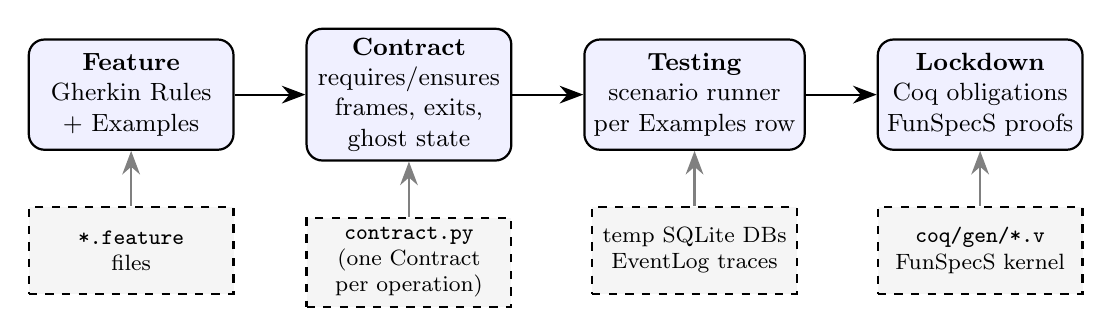
\begin{tikzpicture}[
  stage/.style={draw, rounded corners=2mm, thick, fill=blue!6,
                minimum width=2.6cm, minimum height=1.4cm,
                align=center, font=\small},
  artifact/.style={draw, dashed, thick, fill=gray!8,
                   minimum width=2.6cm, minimum height=1.1cm,
                   align=center, font=\footnotesize},
  arr/.style={-{Stealth[length=3mm]}, thick},
  ]
  \node[stage] (feat) {\textbf{Feature}\\Gherkin Rules\\+ Examples};
  \node[stage, right=0.9cm of feat] (contract) {\textbf{Contract}\\requires/ensures\\frames, exits,\\ghost state};
  \node[stage, right=0.9cm of contract] (test) {\textbf{Testing}\\scenario runner\\per Examples row};
  \node[stage, right=0.9cm of test] (proof) {\textbf{Lockdown}\\Coq obligations\\FunSpecS proofs};

  \node[artifact, below=0.7cm of feat] (fsrc) {\texttt{*.feature}\\files};
  \node[artifact, below=0.7cm of contract] (csrc) {\texttt{contract.py}\\(one Contract\\per operation)};
  \node[artifact, below=0.7cm of test] (tsrc) {temp SQLite DBs\\EventLog traces};
  \node[artifact, below=0.7cm of proof] (psrc) {\texttt{coq/gen/*.v}\\FunSpecS kernel};

  \draw[arr] (feat) -- (contract);
  \draw[arr] (contract) -- (test);
  \draw[arr] (test) -- (proof);
  \draw[arr, gray] (fsrc) -- (feat);
  \draw[arr, gray] (csrc) -- (contract);
  \draw[arr, gray] (tsrc) -- (test);
  \draw[arr, gray] (psrc) -- (proof);
\end{tikzpicture}
\caption{The vericoding pipeline.  Features and contracts are the
primary lasting artifacts; generated code is a replaceable
implementation detail.  Every Examples row is exercised against the
contract; the same contract lowers to Rocq obligations proved against
a hand-verified kernel.}
\label{fig:pipeline}
\end{figure}

\begin{table}[t]
\centering\small
\begin{tabular}{@{}p{0.25\linewidth}p{0.65\linewidth}@{}}
\toprule
\textbf{Stage} & \textbf{What happens} \\
\midrule
\textbf{1. Feature} &
  A Gherkin \texttt{reserve.feature} contains:
  \texttt{Given a product "S1" with on-hand 100 reserved 10 ...}
  with an Examples table of concrete rows. \\[8pt]

\textbf{2. Witness} &
  A pure Python function maps each row to a typed \texttt{ReserveArgs(sku="S1", order\_id="O1", quantity=30)}
  and an initial products dict: \texttt{\{"S1": Product(on\_hand=100, reserved=10, ...)\}}. \\[8pt]

\textbf{3. Materialize} &
  A temp SQLite file is created, DDL run, and rows inserted.  The concrete world is:
  \texttt{Execution\-Context(engine=create\_engine("sqlite:///tmp/..."), events=EventLog())}. \\[8pt]

\textbf{4. Pre-snapshot} &
  \texttt{snapshot(context) $\to$ SpecState}: reads \texttt{products} via SQLAlchemy,
  partitions the empty event log, computes derived totals, and returns an immutable frozen dataclass. \\[8pt]

\textbf{5. Admissibility} &
  \texttt{requires(state, args)} is evaluated: \texttt{args.quantity > 0 $\land$ args.sku $\in$ state.observed.products}.
  If \texttt{outcome = "rejected"}, admissibility is expected to fail; for \texttt{"success"}, it must hold. \\[8pt]

\textbf{6. Invoke service} &
  \texttt{Inventory\-Service().reserve(engine, "S1", "O1", 30)} runs against the real SQLite file through SQLAlchemy.
  On success it returns a \texttt{Reservation\-Receipt}; the effect-emitting wrapper records
  \texttt{StockReserved} and gauge events in the context's event log. \\[8pt]

\textbf{7. Post-snapshot} &
  The \textbf{same} \texttt{snapshot} function runs against the now-mutated SQLite file,
  producing the post-state \texttt{SpecState} with updated reserved count and appended event tuples. \\[8pt]

\textbf{8. Contract check} &
  The runner evaluates: (a) \textbf{frame} --- everything outside \texttt{writes} unchanged;
  (b) \textbf{derives} --- recomputed aggregates consistent;
  (c) \textbf{ensures} --- reserved increased by exactly the quantity, exactly one
  \texttt{StockReserved} event emitted with exact fields;
  (d) \textbf{invariants} --- reserved $\leq$ on-hand, both non-negative. \\[8pt]

\textbf{9. Lower} &
  The same \texttt{Contract} object is introspected by \texttt{specsaver.lower}: deltas,
  scalars, and exception arms are extracted; a Rocq obligation file is emitted.
  \texttt{coqc} compiles it; per-obligation bisection yields a scoreboard. \\[8pt]

\textbf{10. Prove} &
  \texttt{coqc -R coq "" coq/gen/GenReserveObligations.v} succeeds.
  O1--O8 are machine-checked: admissibility sanity, spec consistency, exit coverage,
  invariant preservation, and frame soundness --- all \textsc{proved}. \\
\bottomrule
\end{tabular}
\caption{End-to-end walkthrough of the reserve contract.  Ten stages,
one spec, three levels of assurance.}
\label{tab:walkthrough}
\end{table}

%=====================================================================
\section{Scientific Contributions}\label{sec:contributions}
%=====================================================================

\begin{enumerate}[label=\textbf{C\arabic*}]
\item \textbf{Contracts as semantic intermediate representation.}
  We show that a single declarative contract, written in a restricted
  fragment of Python, serves simultaneously as: an executable test
  oracle over Gherkin scenario data; a generator of semantic frame
  and derived-consistency checks; and the source representation from
  which machine-checked proof obligations are lowered.

\item \textbf{Semantic frame inference.}
  Rather than requiring explicit ``everything else unchanged''
  clauses, declarative write paths over keyed rows, keyed attributes,
  and event channels generate the complement automatically.  The
  checker derives frame soundness from write paths alone.

\item \textbf{Differentially validated library theories.}
  We define a \emph{theory} as a layered operational model of a
  library's covered fragment: action model, event model, state model,
  stub handler, shim adapter, and differential fidelity suite.
  Theories for SQL (SQLAlchemy), logging, and OpenTelemetry are
  built and validated against their real counterparts.

\item \textbf{Symmetric projection architecture.}
  The projection from concrete execution state (SQLite file + event
  log) to abstract specification state is a single function applied
  identically before and after execution, guaranteeing that pre- and
  post-state are comparable under the same interpretation.

\item \textbf{Automatic lowering from executable contracts to Rocq.}
  A shape-extracting introspector analyses the Python AST of each
  contract clause; a shape-driven emitter produces a Rocq obligation
  file targeting a hand-verified WP calculus; a proof harness compiles
  and bisects per obligation.  All four example contracts' store
  obligations are machine-proved.

\item \textbf{Declarative domain specification.}
  A single \texttt{SqlDomain} object collapses per-domain
  infrastructure (materialiser, projection, cleanup, runner wiring,
  test dispatch) into one declaration, reducing a new verification
  unit to its irreducible content.
\end{enumerate}

%=====================================================================
\section{Formal Model}\label{sec:model}
%=====================================================================

Before describing the implementation we fix the semantic objects the
toolchain reasons about.  The state of a system is partitioned into
three strata.

\begin{definition}[Specification state]
$\Sigma = \langle \mathcal{O}, \mathcal{D}, \mathcal{G} \rangle$ where
$\mathcal{O}$ is the \emph{observed state} (a tuple of typed maps and
event-channel tuples read from concrete execution),
$\mathcal{D}$ is the \emph{derived state} (a tuple of pure
computations over $\mathcal{O}$, equipped with a consistency check
$\mathsf{derive}:\mathcal{O}\to\mathcal{D}$),
and $\mathcal{G}$ is \emph{ghost state} (auxiliary specification-only
state invisible to the implementation).
\end{definition}

\begin{definition}[Contract satisfaction]
A contract $C = \langle \Sigma, \mathsf{pre}, \mathsf{post}, \mathcal{X},
\mathcal{I}, \mathcal{W}, \mathcal{R} \rangle$ is \emph{satisfied} by
an execution $\sigma \xrightarrow{a} \sigma'$ with result $r$ (where
$a$ are the call arguments) iff:
\begin{enumerate}[label=(\roman*),nosep]
\item $\mathsf{pre}(\sigma, a)$ holds (admissibility);
\item if no exception condition in $\mathcal{X}$ holds, then
  $\mathsf{post}(\sigma, a, r, \sigma')$ holds, and every state path
  outside $\mathcal{W}$ is unchanged between $\sigma$ and $\sigma'$;
\item if an exception condition $C_i \in \mathcal{X}$ holds, then the
  raised exception matches $E_i$ and every state path outside the
  exit-specific frame $W_i$ is unchanged.
\item $\mathcal{I}(\sigma)$ and $\mathcal{I}(\sigma')$ hold
  (invariants preserved);
\item $\mathsf{derive}(\sigma.\mathcal{O}) = \sigma.\mathcal{D}$ and
  $\mathsf{derive}(\sigma'.\mathcal{O}) = \sigma'.\mathcal{D}$
  (derived consistency).
\end{enumerate}
\end{definition}

\begin{definition}[Semantic frame]
Let $\mathcal{W}$ be a set of \emph{write paths}: strings of the form
$\mathit{map}[key].\mathit{attr}$, $\mathit{map}[key]$, or
$\mathit{channel}$.  For a write path $p \in \mathcal{W}$ whose key
is the argument attribute $k$, the frame checker verifies:
\begin{itemize}[nosep]
\item $\sigma.\mathcal{O}[p] = \sigma'.\mathcal{O}[p]$ for every
  keyed path not in $\mathcal{W}$ (attribute stability);
\item the key sets of every keyed map are equal between $\sigma$ and
  $\sigma'$ except for keyed-row write paths, which may add the
  args-resolved key (insertion) but never delete.
\end{itemize}
\end{definition}

\begin{definition}[Projection symmetry]
A projection $\mathsf{snap}: \mathit{Ctx} \to \Sigma$ is
\emph{symmetric} if it is applied identically before and after
execution: $\sigma^{\mathsf{pre}} = \mathsf{snap}(c)$,
$\sigma^{\mathsf{post}} = \mathsf{snap}(\mathsf{exec}(c))$, and
contract satisfaction is decided over
$(\sigma^{\mathsf{pre}}, a, r, \sigma^{\mathsf{post}})$.
\end{definition}

\begin{definition}[Theory]
A \emph{theory} for a library $L$ is a tuple
$\langle \mathcal{A}, \mathcal{E}, S, H, \mathsf{adapt},
\mathsf{fid} \rangle$ where $\mathcal{A}$ is the action model
(covered fragment of $L$), $\mathcal{E}$ is the event model (trace
entries), $S$ is the pure state model, $H$ is a stub handler
interpreting actions over $S$ and recording a trace,
$\mathsf{adapt}$ connects $H$ to $L$'s API so unmodified service code
runs against the stub, and $\mathsf{fid}$ is a differential test
suite establishing observational equivalence between the stub and $L$
on the covered fragment.
\end{definition}

%=====================================================================
\section{Contract Language}\label{sec:language}
%=====================================================================

A \textsf{specsaver} contract is a first-class Python object built by
the \texttt{Contract} constructor in the \emph{fluid contract} style
\cite{Meyer92,Leino10}: the contract is a declarative value assembled
from named clauses, not imperative assertions scattered throughout the
code.

The contract language is the \textbf{pure terminating fragment of
Python}: every clause is a lambda whose body may contain only
arithmetic, comparison, boolean operators, attribute access, and a
small fixed set of combinator calls (\texttt{extends\_by\_one},
\texttt{implies}, \texttt{safe\_div}).  Side effects, loops,
exceptions, and non-boolean returns are rejected by a static purity
checker before the clause is executed or lowered.  Every clause must
evaluate to a Python \texttt{bool}.

\begin{definition}[Contract record]\label{def:contract}
A contract for an operation is
$\langle \Sigma, \mathit{args}, \mathsf{pre}, \mathsf{post},
\mathcal{X}, \mathcal{I}, \mathcal{D}, \mathcal{W}, \mathcal{R},
\mathcal{G} \rangle$ where:
\begin{itemize}[nosep,leftmargin=*]
\item $\Sigma$ is the specification state type;
\item $\mathit{args}$ is a typed argument record (a frozen dataclass);
\item $\mathsf{pre}(\sigma, a)$ is a boolean predicate (admissibility);
\item $\mathsf{post}(\sigma, a, r, \sigma')$ is a boolean predicate
  (success obligations);
\item $\mathcal{X} = \{\,\langle E_i, C_i, W_i, P_i\rangle \mid i
  \in [1..n] \,\}$ is the set of exceptional exits;
\item $\mathcal{I}$ is the invariant set; $\mathcal{D}$ maps derived
  field names to pure functions; $\mathcal{W}$ and $\mathcal{R}$ are
  the write and read frame path sets; $\mathcal{G}$ carries ghost
  type, initialisation, transitions, and invariants.
\end{itemize}
\end{definition}

\subsection{Semantic frames}

Frame conditions in classical DbC are notoriously verbose.  In
\textsf{specsaver} the contract declares only what it \emph{may}
write:

\[
\mathcal{W} = \{\,
  \text{``state.products[sku].reserved''},\;
  \text{``state.invitations[token]''},\;
  \text{``state.reservation\_log''}
\,\}
\]

The checker derives frame soundness automatically: every attribute
outside $\mathcal{W}$ must be equal, every key outside the
args-resolved write paths must have stable key sets, and deletions are
always rejected.  Keyed-row paths may \emph{add} the args-resolved key
--- essential for operations such as \texttt{invite} that create rows.

\subsection{Exceptional exits}

Exceptions are specified as data:

\[
\mathcal{X} = \bigl\{\,
\langle \mathsf{InsufficientStock},\;
       s.\mathit{available}(a.\mathit{sku}) < a.\mathit{quantity},\;
       \{\mathit{failure\_log}\},\;
       \mathsf{failure\_ensures}
\rangle \,\bigr\}
\]

The runner checks that when the \texttt{when} condition holds, the
correct exception is raised, the exit's frame is respected, and the
failure telemetry contains exactly one new event with the declared
fields.  The classical ``exceptions leave state untouched'' discipline
is the default empty frame.

\subsection{Telemetry: \texttt{extends\_by\_one}}

The combinator $\mathsf{extends\_by\_one}(\mathit{old}, \mathit{new},
\mathit{pred})$ states that $\mathit{new}$ is exactly $\mathit{old}$
with one element appended, and the appended element satisfies
$\mathit{pred}$.  It is the contract language's primitive for
asserting event-channel content, used in both success and exit
post-conditions.  The runtime interpretation is
$|\mathit{new}| = |\mathit{old}| + 1 \land \mathit{new}[:\!-1] =
\mathit{old} \land \mathit{pred}(\mathit{new}[-1])$; the lowering
translates it to a list-append obligation in the generated Rocq.

%=====================================================================
\section{Symmetric Projection}\label{sec:architecture}
%=====================================================================

The bridge between the concrete execution world and the abstract
specification is a single projection function applied twice.

\begin{figure}[t]
\centering
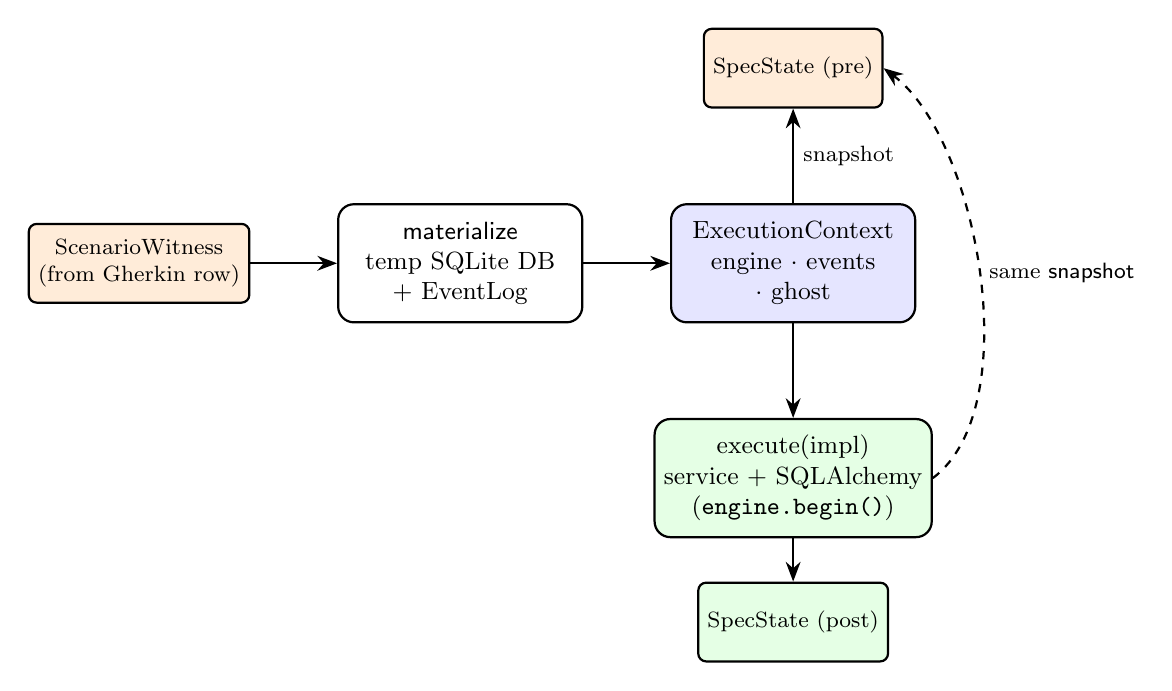
\begin{tikzpicture}[
  box/.style={draw, thick, rounded corners=2mm, minimum width=3.1cm,
              minimum height=1.5cm, align=center, font=\small},
  small/.style={draw, thick, fill=orange!15, rounded corners=1mm,
                minimum width=2.2cm, minimum height=1.0cm,
                align=center, font=\footnotesize},
  arr/.style={-{Stealth[length=2.5mm]}, thick},
  ]
  \node[small] (wit) {ScenarioWitness\\(from Gherkin row)};
  \node[box, right=1.1cm of wit] (mat) {\textsf{materialize}\\temp SQLite DB\\+ EventLog};
  \node[box, right=1.1cm of mat, fill=blue!10] (ctx) {ExecutionContext\\engine $\cdot$ events\\$\cdot$ ghost};
  \node[box, below=1.2cm of ctx, fill=green!10] (impl) {execute(impl)\\service + SQLAlchemy\\(\texttt{engine.begin()})};
  \node[small, above=1.2cm of ctx] (pre) {SpecState (pre)};
  \node[small, below=0.55cm of impl, fill=green!10] (post) {SpecState (post)};

  \draw[arr] (wit) -- (mat);
  \draw[arr] (mat) -- (ctx);
  \draw[arr] (ctx) -- node[right, font=\footnotesize]{snapshot} (pre);
  \draw[arr] (ctx) -- (impl);
  \draw[arr] (impl) -- (post);
  \draw[arr, dashed] (impl.east) .. controls +(1.2,0.9) and +(1.2,-0.9)
        .. node[right, font=\footnotesize]{same \textsf{snapshot}} (pre.east);
\end{tikzpicture}
\caption{The symmetric projection.  \textsf{snapshot(context)} projects
the concrete world both before and after execution; contracts compare
pre and post.  The service is ordinary production code against
SQLAlchemy; the same code runs on a real SQLite file or the theory
stub (\cref{sec:theories}).}
\label{fig:symmetry}
\end{figure}

Given a witness $w$ (from a Gherkin Examples row), the materializer
$M(w)$ produces an execution context: a temp SQLite file, an engine
pointing at it, and a fresh event log.  The scenario runner then
executes a fixed six-stage check per row:
\textsf{materialize}, \textsf{pre-check} (invariants + admissibility),
\textsf{execute} (service + effect-emitting wrapper),
\textsf{frame-check}, \textsf{derived-check},
\textsf{post-check} (ensures + invariants).

Crucially, the service is ordinary production code: SQLAlchemy
\texttt{engine.begin()} transactions, \texttt{text()} statements,
domain exceptions.  Nothing in it knows about contracts, snapshots, or
scenario rows.

%=====================================================================
\section{Examples with Databases}\label{sec:examples}
%=====================================================================

We present three domains of increasing structural interest, all
against SQLite through SQLAlchemy.  \Cref{tab:domains} summarises
their shapes and \cref{tab:metrics} gives quantitative measures.

\subsection{Inventory: deltas and conditional telemetry}

The inventory domain models stock reservations over a single
\texttt{products} table.  Contracts for \texttt{reserve},
\texttt{release}, and \texttt{restock} share the same state schema,
invariants ($0 \leq \mathit{reserved} \leq \mathit{on\_hand}$ for
every product), and derived computations (total on-hand, reserved,
available).

\[
\mathsf{pre}(s, a) \;=\; a.\mathit{quantity} > 0 \;\wedge\; a.\mathit{sku} \in s.\mathit{products}
\]

\[
\mathsf{post}(s, a, r, s') \;=\;
\begin{array}[t]{l}
s'.\mathit{products}[a.\mathit{sku}].\mathit{reserved}
  \;=\; s[\,\cdot\,].\mathit{reserved} + a.\mathit{quantity} \\[2pt]
{}\wedge\; \mathsf{extends\_by\_one}(s.\mathit{reservation\_log},\, s'.\mathit{reservation\_log},\,
      \lambda e.\; e.\mathit{sku} = a.\mathit{sku}) \\[2pt]
{}\wedge\; \mathsf{extends\_by\_one}(s.\mathit{gauge\_log},\, s'.\mathit{gauge\_log},\;
      \lambda g.\; g.\mathit{sku}=a.\mathit{sku} \land g.\mathit{on\_hand}=s'.\mathit{on\_hand}) \\[2pt]
{}\wedge\; \mathsf{implies}(\mathit{crossed}(s,a,s'),\;
      \mathsf{extends\_by\_one}(s.\mathit{alert\_log},\, s'.\mathit{alert\_log},\;
        \ldots))
\end{array}
\]

The alert condition is edge-triggered: available stock crossed from
above the reorder point to at-or-below it.

\subsection{Bank transfer: multi-key deltas and invariants}

The transfer contract moves funds between two rows of one table, with
a balance-nonnegativity invariant and currency-mismatch and
insufficient-funds exits.  Its writes span two different keyed
attributes on different keys, demonstrating that frames compose over
multi-delta operations.

\subsection{Invitations: insertion, multi-table state, and time}

The invitations domain exercises the newest machinery: insert frames,
multi-table acceptance, and time-as-an-argument expiry.

\[
\mathsf{post}_{\mathit{invite}}(s,a,r,s') \;=\;
\begin{array}[t]{l}
s'.\mathit{invitations}[a.\mathit{token}].\mathit{status} = \text{``pending''} \\[1pt]
{}\wedge\; s'.\mathit{invitations}[a.\mathit{token}].\mathit{expires\_at}
       = a.\mathit{now} + 7\!\cdot\!86400
\end{array}
\]

with $\mathcal{W}_{\mathit{invite}} = \{\,\mathit{invitations}[token],\;
\mathit{invite\_log}\,\}$ --- an insert-frame operation.

\[
\mathsf{post}_{\mathit{accept}}(s,a,r,s') \;=\;
\begin{array}[t]{l}
s'.\mathit{invitations}[a.\mathit{token}].\mathit{status} = \text{``accepted''} \\[1pt]
{}\wedge\; s'.\mathit{members}[a.\mathit{user\_id}].\mathit{org\_id}
       = s.\mathit{invitations}[a.\mathit{token}].\mathit{org\_id} \\[1pt]
{}\wedge\; s'.\mathit{users}[a.\mathit{user\_id}].\mathit{default\_org}
       = s.\mathit{invitations}[a.\mathit{token}].\mathit{org\_id}
\end{array}
\]

with $\mathcal{X}_{\mathit{accept}}$ containing
$\mathsf{InvitationExpired}$ (time check) and
$\mathsf{EmailMismatchError}$ (email mismatch) exits.  Token is a
caller-supplied argument so the insert key is args-resolved; expiry
time is an integer epoch so the comparison is pure.

\begin{table}[t]
\centering\small
\begin{tabular}{@{}lcccc@{}}
\toprule
Domain & Tables & Operations & Feature rows & Obligations \\
\midrule
inventory & 1 & reserve, release, restock & 22 & 6/6 $\cdot$ 6/6 $\cdot$ 4/4 \\
bank\_transfer & 2 & transfer & 11 & 7/7 \\
invitations & 3 & invite, accept & 9 & (runtime verification) \\
\bottomrule
\end{tabular}
\caption{The three database-backed example domains.  All feature rows
are exercised by the conformance suite; 23 store obligations across 4
contracts are machine-proved.}
\label{tab:domains}
\end{table}

%=====================================================================
\section{Theories: Library Semantics as Tested Models}\label{sec:theories}
%=====================================================================

A \emph{theory} for a library $L$ is a tuple
$\langle \mathcal{A}, \mathcal{E}, S, H, \mathsf{adapt},
\mathsf{fid} \rangle$ as defined in \cref{sec:model}.  The key
property is that the stub handler is validated by
\emph{differential testing}: the same program runs against the real
library $L$ and against the stub, and their observable outputs must
agree on the covered fragment.

\begin{figure}[t]
\centering
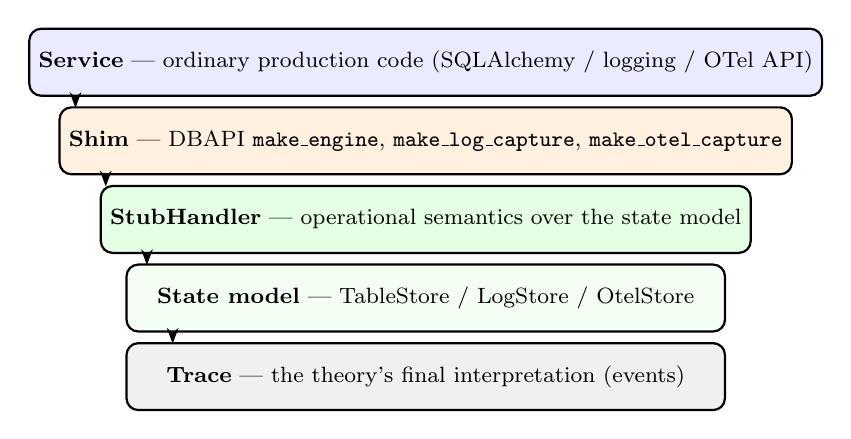
\begin{tikzpicture}[
  layer/.style={draw, thick, rounded corners=1.5mm,
                minimum width=7.6cm, minimum height=0.85cm,
                align=left, font=\footnotesize, anchor=west},
  note/.style={font=\footnotesize\itshape, text=gray!60!black},
  ]
  \node[layer, fill=blue!8] (service) {\textbf{Service} --- ordinary
    production code (SQLAlchemy / logging / OTel API)};
  \node[layer, below=0.12cm of service, fill=orange!12] (shim)
    {\textbf{Shim} --- DBAPI \texttt{make\_engine},
     \texttt{make\_log\_capture}, \texttt{make\_otel\_capture}};
  \node[layer, below=0.12cm of shim, fill=green!10] (handler)
    {\textbf{StubHandler} --- operational semantics over the state model};
  \node[layer, below=0.12cm of handler, fill=green!5] (model)
    {\textbf{State model} --- TableStore / LogStore / OtelStore};
  \node[layer, below=0.12cm of model, fill=gray!12] (trace)
    {\textbf{Trace} --- the theory's final interpretation (events)};

  \draw[-{Stealth[length=2mm]}] (service.south west) ++(0.6,0) -- ++(0,-0.14);
  \draw[-{Stealth[length=2mm]}] (shim.south west) ++(0.6,0) -- ++(0,-0.14);
  \draw[-{Stealth[length=2mm]}] (handler.south west) ++(0.6,0) -- ++(0,-0.14);
  \draw[-{Stealth[length=2mm]}] (model.south west) ++(0.6,0) -- ++(0,-0.14);
\end{tikzpicture}
\caption{The theory stack.  The service is written once, against the
real library API; the shim connects to the stub; the stub interprets
actions over a pure state model and records the trace.  Differential
tests run the same programs against stub and real library and require
identical observable behaviour.}
\label{fig:theory-stack}
\end{figure}

\subsection{SQL theory}

The SQL theory covers a deliberately small fragment: equality-\textsc{where}
\texttt{SELECT} (with ascending \texttt{ORDER BY}), single-row
\texttt{INSERT}, and \texttt{UPDATE} with \texttt{SET col = col $\pm$
expr}.  Statements are parsed by \texttt{sqlglot}; anything outside
the fragment raises \texttt{UnsupportedStatementError} --- no silent
degradation.  The stub handler interprets the action model over an
immutable \texttt{TableStore}, records the trace, and enforces
transaction discipline.  A PEP-249 DBAPI shim exposes the handler so
\emph{unmodified SQLAlchemy service code runs against the theory}.
The sqlite dialect's deferred-autobegin semantics is modelled at the
connection level; \texttt{commit()} and \texttt{rollback()} are, as in
real sqlite3, no-ops without an open transaction.

\subsection{Logging and OpenTelemetry}

The same six-layer shape repeats for logging and OpenTelemetry
theories.  Both ship differential fidelity suites that compare stub
output against the real library.  The logging theory captures every
\texttt{logger.info/warning/error} call as a structured
\texttt{LogEmit} record; the OTel theory captures the full span
lifecycle as a \texttt{SpanRecord}.

\begin{principle}[Theory conformance]
A theory is admissible only if: (i) its stub and the real library
agree observationally on a differential suite; (ii) its translator
rejects out-of-fragment input loudly; (iii) its state model and trace
are pure data.  New theories follow the same checklist.
\end{principle}

%=====================================================================
\section{Domain Declarations}\label{sec:domains}
%=====================================================================

Experience with three domains revealed a stable shape: only types,
service, contracts, features, and witness builders are genuinely
domain content; everything else was byte-identical infrastructure
copied per domain.  The \texttt{SqlDomain} declaration collapses the
latter.

\begin{figure}[t]
\centering
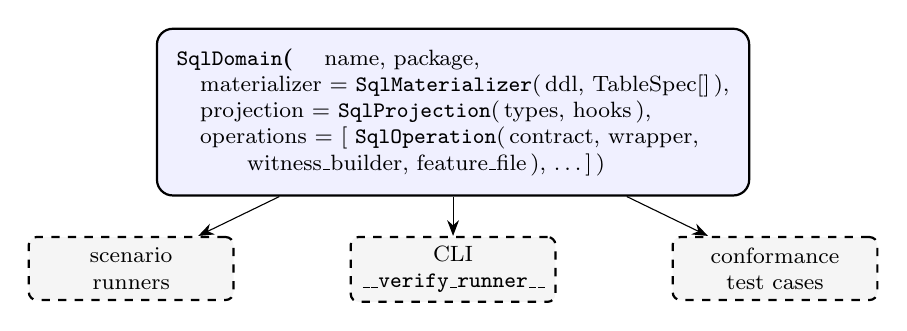
\begin{tikzpicture}[
  decl/.style={draw, thick, fill=blue!6, rounded corners=2mm,
               minimum width=6.6cm, align=left, font=\footnotesize,
               inner sep=2.5mm},
  gen/.style={draw, dashed, thick, fill=gray!8, rounded corners=1mm,
              minimum width=2.6cm, minimum height=0.8cm,
              align=center, font=\footnotesize},
  ]
  \node[decl] (d) {\textbf{\texttt{SqlDomain}(}
    \quad name, package,\\
    \quad materializer = \texttt{SqlMaterializer}(\,ddl, TableSpec[]\,),\\
    \quad projection = \texttt{SqlProjection}(\,types, hooks\,),\\
    \quad operations = [ \texttt{SqlOperation}(\,contract, wrapper,\\
    \quad\qquad witness\_builder, feature\_file\,), \ldots ]\,)};
  \node[gen, below left=0.5cm and -1.0cm of d] (r1) {scenario\\runners};
  \node[gen, below=0.5cm of d] (r2) {CLI\\\texttt{\_\_verify\_runner\_\_}};
  \node[gen, below right=0.5cm and -1.0cm of d] (r3) {conformance\\test cases};
  \draw[-{Stealth[length=2mm]}] (d) -- (r1);
  \draw[-{Stealth[length=2mm]}] (d) -- (r2);
  \draw[-{Stealth[length=2mm]}] (d) -- (r3);
\end{tikzpicture}
\caption{One \texttt{SqlDomain} declaration derives runners, CLI
dispatch, and the conformance suite.}
\label{fig:domain-decl}
\end{figure}

A \texttt{TableSpec} names a table's columns, primary key, and the
witness attribute carrying its initial rows; from these the
materializer generates DDL execution, \texttt{DELETE + INSERT}
seeding, engine construction, and teardown.  The projection queries
each declared table and passes row dicts plus the event log to two
small domain hooks.  Domains with irregular tables declare a
\texttt{populate\_extra} hook.

%=====================================================================
\section{Lowering Architecture}\label{sec:lowering}
%=====================================================================

The lowering pipeline transforms a Python \texttt{Contract} into a
Rocq obligation file and scores each obligation against a
hand-verified kernel.  The pipeline has three stages:
\textsf{introspect}, \textsf{emit}, and \textsf{score}.

\begin{figure}[t]
\centering
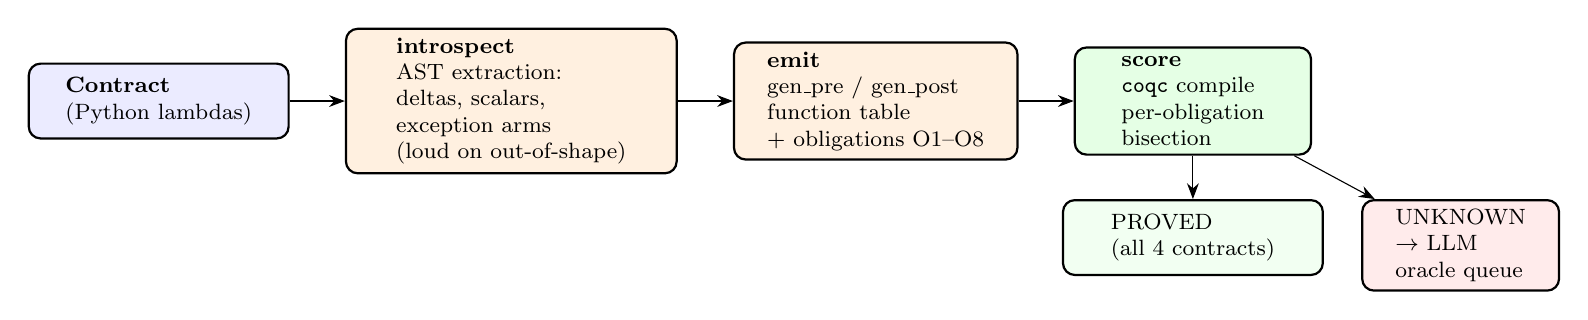
\begin{tikzpicture}[
  node/.style={draw, thick, rounded corners=1.5mm, minimum height=0.95cm,
               align=left, font=\footnotesize, anchor=west},
  ]
  \node[node, fill=blue!8, minimum width=3.3cm] (c) {\textbf{Contract}\\(Python lambdas)};
  \node[node, fill=orange!12, minimum width=4.2cm, right=0.7cm of c]
        (i) {\textbf{introspect}\\AST extraction:\\deltas, scalars,\\exception arms\\(loud on out-of-shape)};
  \node[node, fill=orange!12, minimum width=3.6cm, right=0.7cm of i]
        (e) {\textbf{emit}\\gen\_pre / gen\_post\\function table\\+ obligations O1--O8};
  \node[node, fill=green!10, minimum width=3.0cm, right=0.7cm of e]
        (s) {\textbf{score}\\\texttt{coqc} compile\\per-obligation\\bisection};
  \node[node, fill=green!5, minimum width=3.3cm, below=0.55cm of s] (ok)
        {PROVED\\(all 4 contracts)};
  \node[node, fill=red!8, minimum width=2.5cm, below=0.55cm of s, xshift=3.4cm]
        (unk) {UNKNOWN\\$\to$ LLM\\oracle queue};
  \draw[-{Stealth[length=2mm]}] (c) -- (i);
  \draw[-{Stealth[length=2mm]}] (i) -- (e);
  \draw[-{Stealth[length=2mm]}] (e) -- (s);
  \draw[-{Stealth[length=2mm]}] (s) -- (ok);
  \draw[-{Stealth[length=2mm]}] (s) -- (unk);
\end{tikzpicture}
\caption{The lowering pipeline: introspect, emit, score.}
\label{fig:lowering}
\end{figure}

\subsection{The Rocq kernel}

The Coq side comprises three layers.  \textbf{SnakeletExnLang} is a
small imperative language with dictionaries, lists, exceptions, and an
evaluation relation.  \textbf{SnakeletExnWp} provides a
weakest-precondition calculus over it with stateful opaque
specifications.  \textbf{SpecPrelude} provides dictionary
lookup/insert helpers and their correctness lemmas, proven once rather
than per contract.

The specification kernel (\textbf{FunSpecS}) maps operation names to
stateful specs $(\mathit{pre}, \mathit{post})$ where
$\mathit{post}(\sigma, vs, r, \mathit{ups})$ constrains the result $r
\in \{\,\mathsf{RVal}(v), \mathsf{RExn}(\ell, p)\,\}$
and the list of heap-cell updates $\mathit{ups}$.  The kernel
guarantees that each spec is total: for every pre-state $\sigma$ and
argument list $vs$ satisfying $\mathit{pre}(\sigma, vs)$, there exist
a result $r$ and updates $\mathit{ups}$ satisfying
$\mathit{post}(\sigma, vs, r, \mathit{ups})$ and respecting the map
domain.

\subsection{Shape extraction (introspect)}

The introspector (\texttt{introspect.py}) parses each clause's Python
AST into a \texttt{ContractInfo} shape object:

\begin{itemize}[nosep]
\item \textbf{Deltas}: expressions of the form
  $\mathit{new}.\mathit{map}[\mathit{key}].\mathit{field}
  = \mathit{old}.\mathit{map}[\mathit{key}].\mathit{field} \pm
  \mathit{args}.\mathit{qty}$ are extracted as
  $(\mathit{key}, \mathit{field}, op, \mathit{qty})$ tuples.
\item \textbf{Scalars}: simple comparisons ($\mathit{args}.x > 0$,
  $\mathit{args}.x \neq \mathit{args}.y$) are reduced to
  $(\mathit{lhs}, op, \mathit{rhs})$ triples.
\item \textbf{Exceptions}: the class name, conjunctive when-conditions,
  and payload fields are extracted.
\item \textbf{Traces}: \texttt{extends\_by\_one} calls are detected
  and deferred to a later lowering pass.
\item \textbf{Out-of-shape rejection}: anything not matching the
  supported fragment raises \texttt{UnsupportedShapeError}.  Every
  clause is gate-checked for purity.
\end{itemize}

\subsection{Emission}

The emitter (\texttt{emit.py}) translates a \texttt{ContractInfo} into
a complete Rocq file.  The generated structure per operation is:

\begin{itemize}[nosep]
\item \textbf{Heap model}: two locations,
  $\mathit{store\_loc}$ (the table dict) and $\mathit{trace\_loc}$
  (the event dict).
\item \textbf{Row constructors}: $\mathsf{row\_of}(f_1, \dots, f_k)$
  builds a \texttt{LitDict} with typed fields.
\item \textbf{Row invariant}: $\mathsf{row\_inv}(v)$ holds iff there
  exist fields such that $v = \mathsf{row\_of}(\dots)$ and the
  invariant conjuncts hold (e.g.\ non-negativity, ordering).
\item \textbf{Store invariant}: $\mathsf{store\_inv(kvs)}$ lifts
  $\mathsf{row\_inv}$ over all entries.
\item \textbf{Pre/post}: $\mathsf{gen\_pre}$ and $\mathsf{gen\_post}$
  bind all free variables existentially, look up each key's row via
  $\mathsf{dict\_lookup\_str}$, conjunct the scalar preconditions, and
  (for post) describe the result and the \emph{nested insert} of all
  deltas.
\item \textbf{Function table}: $\mathsf{gen\_table}$ maps operation
  names to $\mathsf{FunSpecS}$ entries, with one arm per exception
  exit.
\item \textbf{Totality lemmas}: $\mathsf{gen\_table\_total}$ and
  $\mathsf{gen\_table\_total\_pure}$ prove that the table satisfies
  the $\mathsf{FunCtx}$ requirements.
\item \textbf{Per-delta preservation}: each delta gets a lemma showing
  the store invariant survives the single-row update.
\end{itemize}

\begin{lstlisting}[style=coq]
Definition gen_post (sigma : sn_state) (vs : list sn_val)
    (r : Result) (ups : cell_updates) : Prop :=
  exists sku order quantity store_d on_hand_sku
         reserved_sku reorder_point_sku,
    vs = [LitString sku; LitString order; LitInt quantity] /\
    sigma !! store_loc = Some (LitDict store_d) /\
    dict_lookup_str sku store_d =
      Some (row_of on_hand_sku reserved_sku reorder_point_sku) /\
    r = RVal (LitInt reserved_sku) /\
    ups = [(store_loc, LitDict (dict_insert_str sku
            (row_of on_hand_sku (reserved_sku + quantity)
                    reorder_point_sku) store_d))].
\end{lstlisting}

\subsection{Obligation set}

The generated file contains eight numbered obligations:

\begin{tabular}{@{}lp{0.7\linewidth}@{}}
\toprule
\textbf{Obligation} & \textbf{Statement} \\
\midrule
O1 & Admissibility sanity: $\exists \sigma, vs.\;
     \mathsf{gen\_pre}(\sigma, vs) \land \mathsf{store\_inv}(\sigma)$
     --- the spec is non-vacuous. \\
O2 & Spec consistency: $\mathsf{gen\_pre}(\sigma, vs) \implies
     \exists r, \mathit{ups}.\; \mathsf{gen\_post}(\sigma, vs, r, \mathit{ups})
     \land \mathsf{updates\_dom\_in}(\sigma, \mathit{ups})$
     --- the success path is reachable. \\
O3.$i$ & Each exception arm is satisfiable: given its pre, there
          exists a result and updates satisfying its post. \\
O4 & Exit coverage: the success availability and the disjunction of
     all exit when-conditions partition the state space. \\
O5 & Invariant preservation across all nested delta updates. \\
O8 & Frame soundness: for any location $l \neq \mathsf{store\_loc}$,
     $\mathsf{apply\_updates}(\sigma, \mathit{ups}) !! l \;=\; \sigma !! l$. \\
\bottomrule
\end{tabular}

\subsection{Proof harness}

\texttt{harness.py} first compiles the whole file with
\texttt{coqc}.  If the whole-file compile succeeds, every obligation
is labelled \textsc{proved}.  On failure, it \emph{bisects}: for each
obligation lemma, it generates a variant file where every other lemma
is replaced with \texttt{Proof. Admitted.}, then compiles the variant
in isolation.  Obligations that compile in isolation are
\textsc{proved}; the remainder are \textsc{unknown}, packaged as
self-contained proof problems for an LLM-based oracle.

A third status, \textsc{disproved}, is the natural extension when a
runtime check fails: the scenario runner already exercises every
contract clause against concrete data, and a counterexample for a
well-formed contract means the specification is inconsistent.

%=====================================================================
\section{Trusted Computing Base}\label{sec:tcb}
%=====================================================================

The following components are \textbf{trusted} (not themselves
machine-proved):

\begin{itemize}[nosep]
\item The Rocq kernel and the \texttt{coqc} proof checker.
\item The \texttt{FunSpecS} kernel and \texttt{SnakeletExnWp}
  calculus: hand-written Rocq that must correctly model the intended
  operational semantics.
\item The \texttt{SpecPrelude} dictionary helpers.
\item The lowering implementation itself: \texttt{introspect.py} (AST
  extraction and shape recognition), \texttt{emit.py} (translation to
  Rocq), \texttt{frames.py} (frame checking), and \texttt{purity.py}
  (static purity validation).
\end{itemize}

\noindent The following are \textbf{proved} by the generated obligations:
admissibility non-vacuity, post-state consistency, exit coverage,
invariant preservation, and frame soundness -- relative to the kernel.

\noindent The following are \textbf{not yet proved}:
refinement between the Coq model and the concrete Python
implementation (the scenario runner tests this empirically); trace
obligations in the lowering; and the correctness of the emitter itself.

%=====================================================================
\section{Evaluation}\label{sec:evaluation}
%=====================================================================

\begin{table}[t]
\centering\small
\begin{tabular}{@{}lr@{}}
\toprule
\textbf{Metric} & \textbf{Value} \\
\midrule
Python source lines (specsaver core + examples) & $\approx$ 10,000 \\
Rocq source lines (kernel + proofs) & $\approx$ 3,500 \\
Number of example domains & 3 \\
Number of contracts & 6 \\
Number of feature rows exercised & 42 \\
Generated obligations per contract & 4--8 \\
Store obligations proved & 23/23 \\
Trace obligations (runtime only) & deferred \\
Runtime verification per row & $< 0.1$\,s \\
Lowering time (introspect + emit) & $< 0.5$\,s per contract \\
Rocq compilation per obligation file & $< 30$\,s \\
\bottomrule
\end{tabular}
\caption{Quantitative measures of the \textsf{specsaver} implementation.
All store obligations are machine-proved.}
\label{tab:metrics}
\end{table}

\Cref{tab:metrics} gives quantitative measures.  All 23 store
obligations across four contracts are fully proved against the Rocq
kernel.  Trace obligations (list-append post-conditions for event
channels) are enforced at runtime by the scenario runner and are the
active development front in the lowering.

The three example domains exercise a range of verification scenarios:
single-table keyed deltas (inventory), multi-key deltas with a
conservation invariant (bank transfer), and insert-frame multi-table
deltas with time-based exception exits (invitations).  All 42 feature
rows are exercised by the generic conformance suite.

\subsection{Implemented versus future work}

The following are \textbf{implemented} and operational: executable
contracts with pre/post conditions and exception exits; semantic frame
checking; runtime scenario verification; domain declarations with
generic conformance testing; the SQL, logging, and OpenTelemetry
theories with differential fidelity suites; the lowering pipeline with
shape extraction, emission, and proof scoring; and all 23 store
obligations machine-proved.

The following are \textbf{future work}: trace-cell obligations in the
lowering; user-supplied ghost algebras; incremental re-verification
keyed on contract/body hashes; loop and sequence support in the
obligation generator; DISPROVED counterexample surfacing; and
expanding the supported language fragment.

%=====================================================================
\section{Related Work}\label{sec:related}
%=====================================================================

\begin{itemize}[leftmargin=*]

\item \textbf{Design by Contract} (Meyer~\cite{Meyer92}, Eiffel):
provides runtime assertions without a path to mechanised proof.
\textsf{specsaver} keeps the executable-contract ergonomics and adds
the lowering to Rocq, plus frame inference that eliminates the
verbosity of manual frame conditions.

\item \textbf{Spec\#} (Leino and M\"uller~\cite{Leino10}): a
language-integrated contract system with static verification via
Boogie.  Like Spec\#, \textsf{specsaver} treats contracts as
first-class; unlike Spec\#, the contracts are not tied to the
implementation language and persist independently of the code.

\item \textbf{Dafny, Frama-C, KeY, Why3}: verify source-level
contracts but require the source language to be the specification
language.  \textsf{specsaver} instead verifies an abstract model
aligned with the declared frame, keeping production code unmodified
and language-agnostic.

\item \textbf{Iris separation logic} (Jung et al.): provides a
framework for building WP calculi.  \textsf{specsaver} uses the Iris
\texttt{gen\_heap} library as infrastructure for its Rocq kernel and
shares the heap-cell update model.

\item \textbf{Property-based testing} (QuickCheck~\cite{QuickCheck},
Hypothesis): generates random inputs and checks properties.
\textsf{specsaver} contracts are simultaneously the property oracle
and the proof input; the Gherkin tables provide the concrete test
data.

\item \textbf{Behaviour-driven development} (Gherkin~\cite{Gherkin}):
specifies behaviour in scenario tables.  \textsf{specsaver} connects
Gherkin to executable contracts and formal proof, so the scenarios
become verified test data.

\item \textbf{TLA\textsuperscript{+}}: specifies systems in temporal
logic.  \textsf{specsaver} targets operational semantics and
explicit state transitions with a considerably lower barrier to entry
(Python lambdas vs.\ TLA\textsuperscript{+} formulas).

\end{itemize}

%%=====================================================================
%\section{Threats to Validity and Limitations}\label{sec:threats}
%%=====================================================================

\noindent\textbf{Internal validity.}
The lowering pipeline is trusted code: the emitter's translation from
\texttt{ContractInfo} to Rocq is not itself proved correct.  The frame
checker and purity validator are similarly trusted.  The semantic
object of the proof is the contract, not the implementation --- the
scenario runner tests the latter empirically.

\noindent\textbf{External validity.}
The three example domains are small but representative of
database-backed services: they exercise single-table, multi-table,
insert-bearing, and time-bearing patterns.  The theory mechanism has
been demonstrated for three libraries (SQL, logging, OTel) but the
approach to adding new theories is manual.

\noindent\textbf{Construct validity.}
The claim that contracts form a ``semantic intermediate language'' is
currently instantiated via a specific AST extraction and lowering
pipeline.  The contract fragment is restricted to what the introspector
and emitter can handle; expanding the fragment is future work.

%=====================================================================
\section{Conclusion}\label{sec:conclusion}
%=====================================================================

This paper has presented the thesis that executable behavioural
contracts form a semantic intermediate language from which testing,
runtime checking, differential validation, and machine-checked proof
obligations can all be derived.  A vericoding workflow leaves the
specification as the lasting artifact and the code as a replaceable
implementation detail.

The \textsf{specsaver} toolchain operationalises this thesis through
six contributions: contracts as semantic intermediate representation,
semantic frame inference, differentially validated library theories, a
symmetric projection architecture, automatic lowering to Rocq proof
obligations, and declarative domain specification.  The implementation
is not a proposal --- it exists, it works, and the evidence is
machine-checked: 23 store obligations across four contracts are proved
against a hand-verified WP calculus.

%=====================================================================
\begin{thebibliography}{10}

\bibitem{Meyer92}
Bertrand Meyer.
\textit{Applying ``Design by Contract''}.
IEEE Computer, 25(10):40--51, 1992.

\bibitem{Leino10}
K.\ Rustan M.\ Leino and Peter M\"uller.
\textit{Using the Spec\# Language, Methodology, and Tools to Write
Bug-Free Programs}.
In LASER Summer School 2008/2009, LNCS 6029, Springer, 2010.

\bibitem{SpecSaver25}
Gavin Mendel-Gleason.
\textit{specsaver: Specification-Driven Verification}.
Source code and documentation. \texttt{https://github.com/scidonia/specsaver}, 2025--2026.

\bibitem{Gherkin}
Cucumber Ltd.
\textit{Gherkin Reference}.
\texttt{https://cucumber.io/docs/gherkin/reference/}, 2025.

\bibitem{QuickCheck}
Koen Claessen and John Hughes.
\textit{QuickCheck: A Lightweight Tool for Random Testing of Haskell Programs}.
In ICFP 2000.

\bibitem{SepLogic}
John C.\ Reynolds.
\textit{Separation Logic: A Logic for Shared Mutable Data Structures}.
In LICS 2002.

\bibitem{FunSpecS}
Scidonia.
\textit{SnakeletExn and FunSpecS: A Small Imperative Language and
Weakest-Precondition Specification Kernel}.
Coq development, 2026.

\bibitem{Iris}
Ralf Jung, Robbert Krebbers, Jacques-Henri Jourdan, et al.
\textit{Iris: Monoids and Invariants as an Orthogonal Basis for
Concurrent Reasoning}.  In POPL 2018.

\end{thebibliography}

\end{document}
